\chapter{Literature Review}
\section{Background}

\subsection{Retrieval-augmented Generation (RAG)}
Retrieval-augmented generation (RAG), first introduced by \autocite{lewis2021retrievalaugmentedgenerationknowledgeintensivenlp}, is a method used to enhance the text generation abilities of LLMs.

It is seeing increased usage in multiple LLM-applications, such as medical chat-bots \autocite{jin2024healthllmpersonalizedretrievalaugmenteddisease}, as well as systems for detecting vulnerabilities in code \autocite{du2024vulragenhancingllmbasedvulnerability}.

The widespread adoption of RAG is due to its flexibility; A pre-trained model can be made to function in different domains simply by making adjustments to its RAG components, bypassing the need for extensive re-training.

Furthermore, numerous advancements are being made in enhancing the capabilities of RAGs, such as advanced techniques that improve retrieval qualities, or modular architectures that allow for specific fine-tuning of RAG components \autocite{gao2024retrievalaugmentedgenerationlargelanguage}.

\begin{figure}
	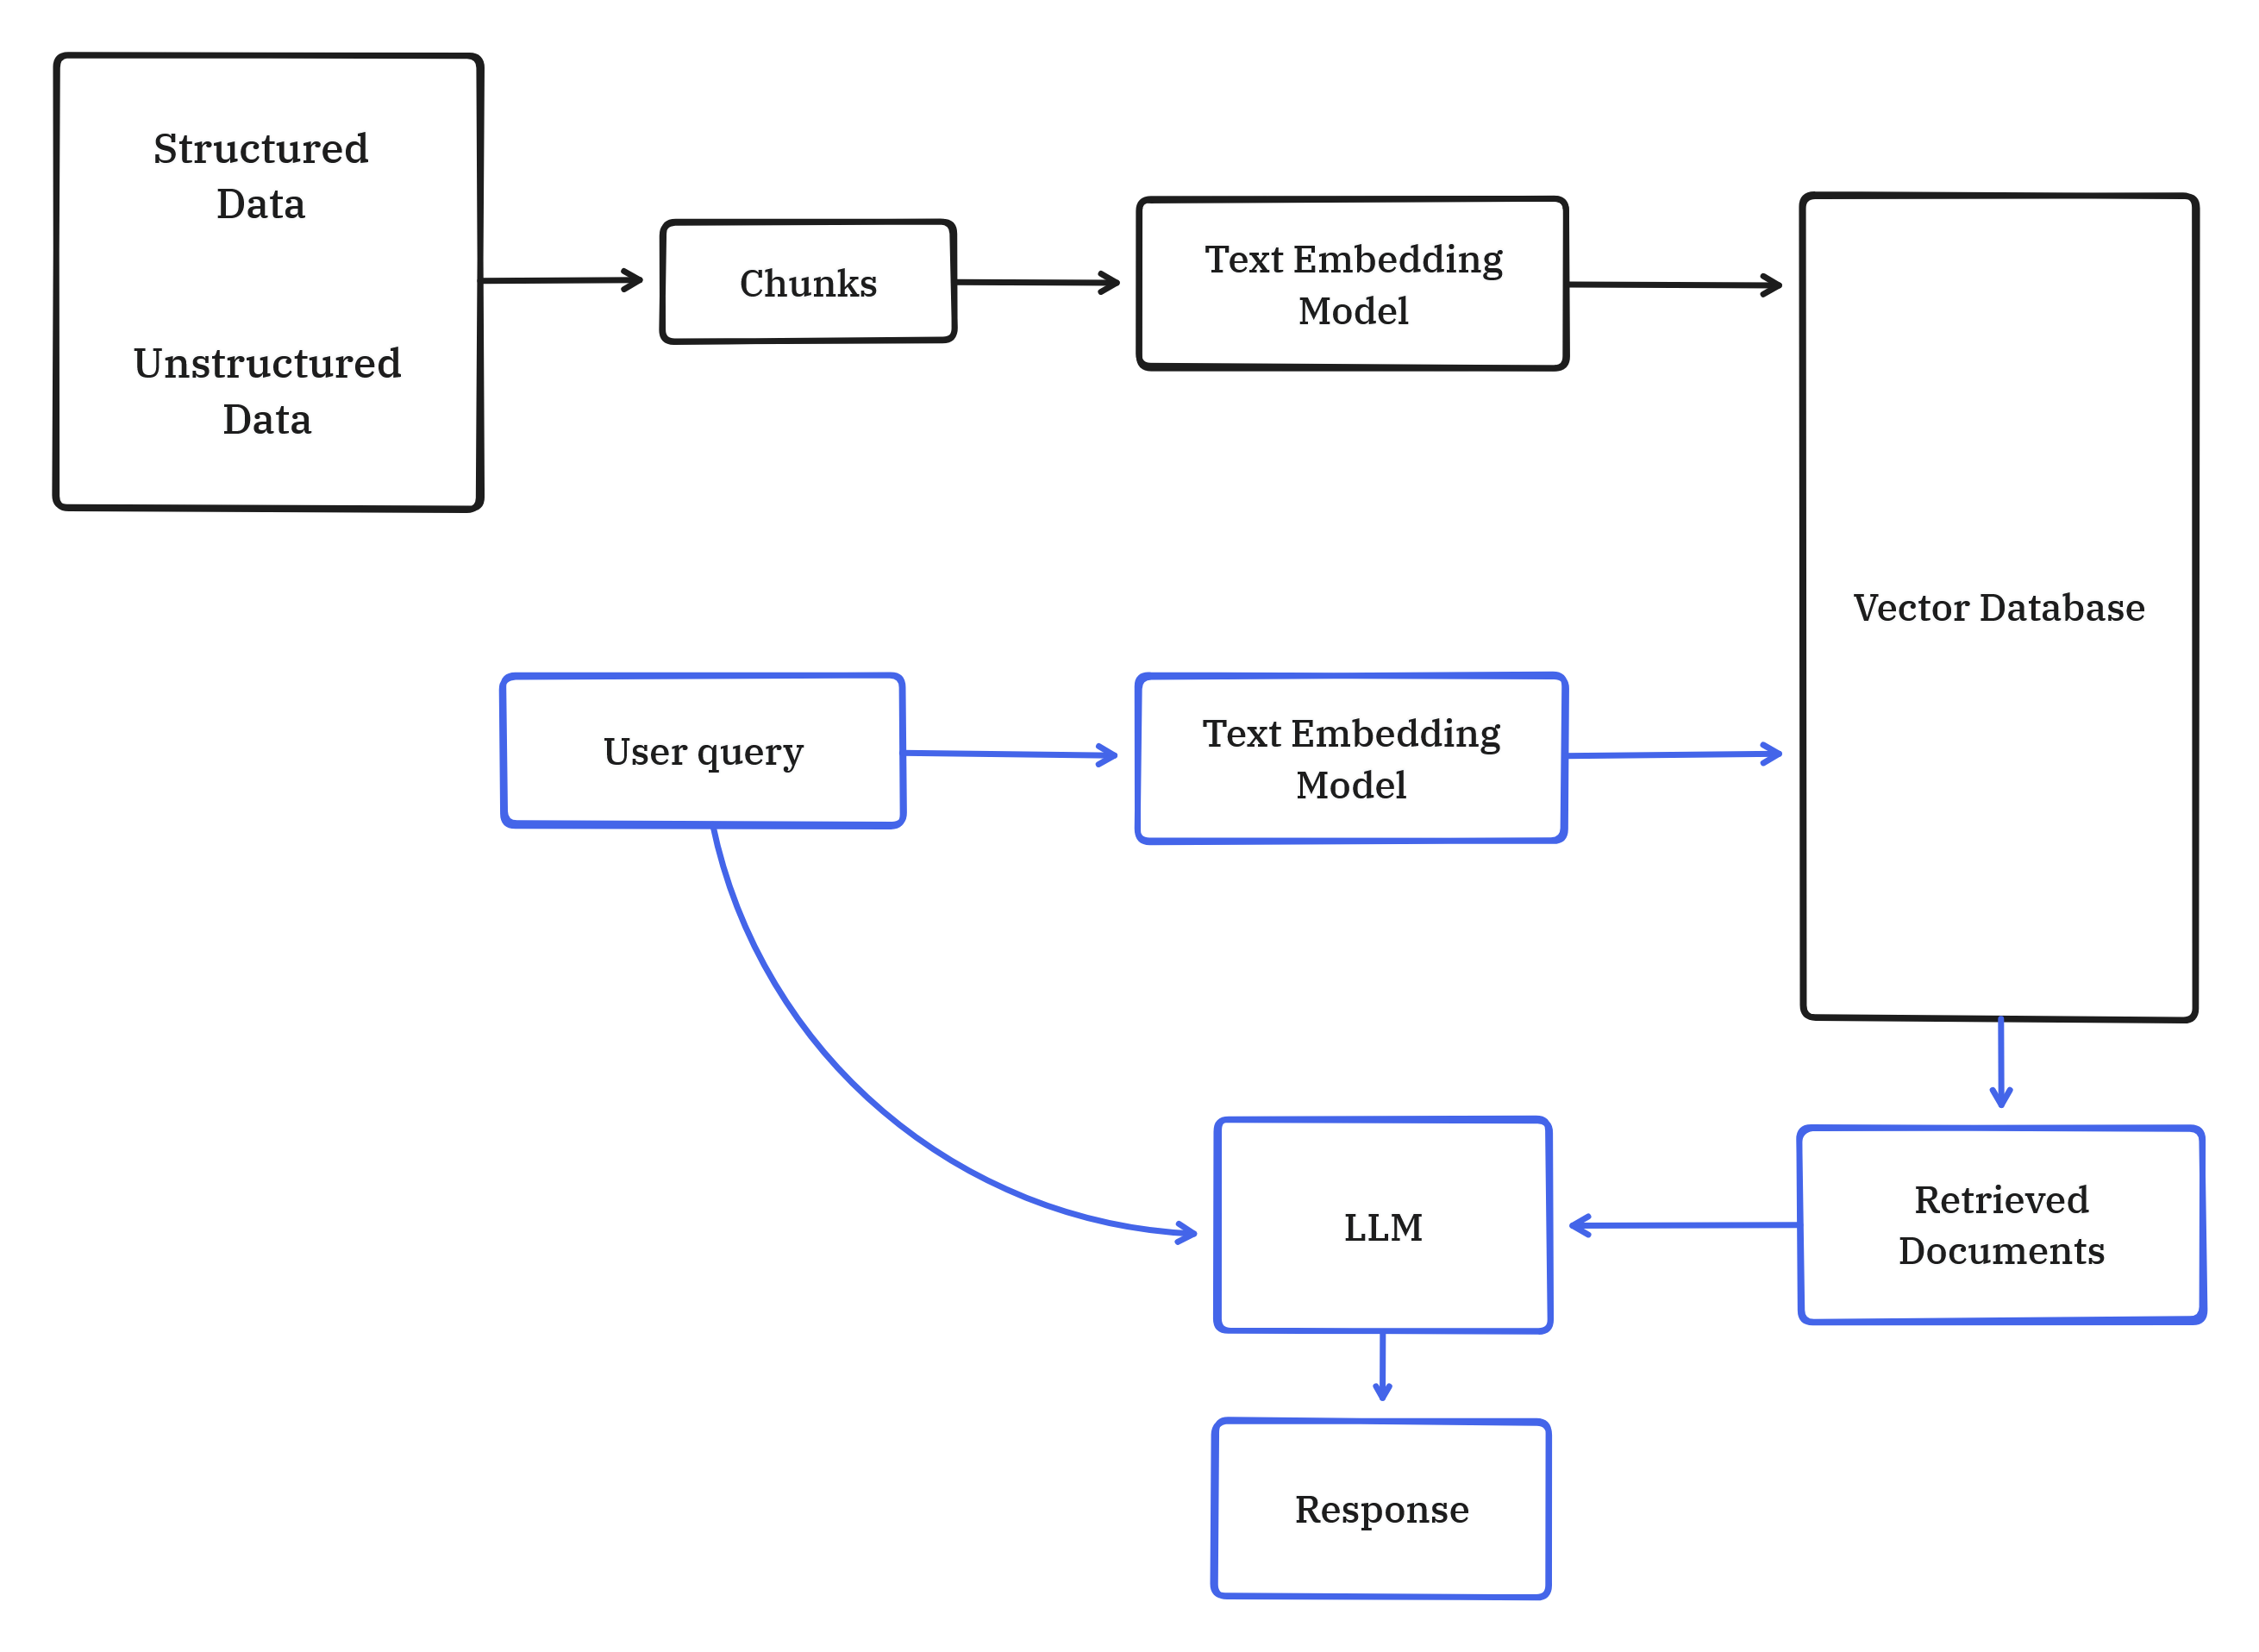
\includegraphics[width=\textwidth]{Conventional RAG example.png}
	\caption{Example of a Conventional RAG system}
	\centering
	\label{fig:RAGexample}
\end{figure}

\subsection{Exploitation of RAG Systems}
Studies (\cite{tan2024gluepizzaeatrocks}; \cite{zeng2024goodbadexploringprivacy}; \cite{xue2024badragidentifyingvulnerabilitiesretrieval}) have shown that RAG systems are susceptible to well-crafted prompt attacks during the retrieval stage.

By using targeted as well as untargeted attacks \autocite{zeng2024goodbadexploringprivacy}, a malicious attacker is able to retrieve personally identifiable information (PII), such as phone numbers and addresses, from a RAG's corpus.


\autocite{tan2024gluepizzaeatrocks} and \autocite{xue2024badragidentifyingvulnerabilitiesretrieval} showcase the ability to affect an LLMs output by inserting specially crafted adversarial passages into its RAG corpus.

This typically affects LLMs that make use of real-time context databases, such as a search engine, which allows an attacker to insert malicious documents into the context database.

\subsection{Large Language Model (LLM) Safeguards}
The widespread usage of LLMs necessitates the development of safeguards to prevent ethical misuse and abuse.
These safeguards are often times complex, varying based on application requirements.

\autocite{dong2024buildingguardrailslargelanguage} discusses the different components involved in implementing guard rails for LLMs and touches on some of the currently deployed solutions available.
In general, safeguards are designed to prevent the LLMs from generating unintended output.
This unintended output can be generated in numerous ways, most notably through ``hallucinations'' as well as targeted prompt attacks known as ``jailbreaking''.
